%!TEX root = ../main.tex
% file: assignment2.tex


\graphicspath{{C:/Documents and Settings/amcelhinney/My Documents/GitHub/MCS507ProjectTwo/tex/include/}}

\section{Assignment Two: Using the Software from Python and Extending Illustrative Example} % (fold)
\label{sec: First}
Our second objective is to review how to utilize this software from Python. We then extend the illustrative example from Assignment One to further display the advantages and disadvantages of the Earth software.

\subsection{Utilizing the Earth Software from Python} % (fold)
\label{sub:methoda}
The Earth software is created by Stephen Milborrow and runs in an R environment. R is an open source enviroment for statistical computer. Interestingly, the R language is an extension of a language developed at Bell Laboratories in the late 1970's and early 1980's. Although the Earth software runs in R, it is also available as a standalone program and as a C library. 

Access to the Earth software from Python is done via the Orange module, which is a module focused on data mining and machine learning. It is also available as a standalone software program complete with a GUI. The Orange module and software is developed by the Bioinformatics Laboratory at the Faculty of Computer and Information Science in the University of Ljubljana, Slovenia (Orange Documentation, 10/20/2012). In addition to the implementation of the Earth software, the Orange module features implementations of the majority of cutting-edge machine learning and data mining techniques, including techniques from the following categories:

\begin{enumerate}
\item Summary Statistics
\item Classification
\item Regression
\item Ensemble Algorithms
\item Clustering
\item Network Analysis
\end{enumerate}

\subsection{Extending the Illustrative Example} 

We now seek to extend our Illustrative Example from Assignment One. The natural question arries, "How does the Earth software compare with other traditional techniques?" To answer this question, we utilize the \emph{polyfit} functions from the \emph{NumPy} module to fit polynomial functions of the 3rd, 4th and 5th degrees. We then plot the predicted versus actual values and compare them to the Earth software.

\begin{lstlisting}[caption={Fit Polynomial Functions of the 3rd, 4th and 5th Degrees.  },label=lst:expected_times,firstnumber=43]
p3=polyfit(x,y,3)
pp3=poly1d(p3)

p4=polyfit(x,y,4)
pp4=poly1d(p4)

p5=polyfit(x,y,5)
pp5=poly1d(p5)

pl.plot(X, Y, ".r")
pl.plot(linspace, predictions, "-b")
pl.plot(linspace,pp3(linspace),"-g")
pl.plot(linspace,pp4(linspace),"-m")
pl.plot(linspace,pp5(linspace),"-y")
pl.title('Example Data Set with Line Fit by MARS and Higher Order Polynomials')
pl.legend(['Data','Mars','3rd Degree','4th Degree','5th Degree'],loc=2)
pl.show()
\end{lstlisting}
\begin{figure}[H]
    \centering
       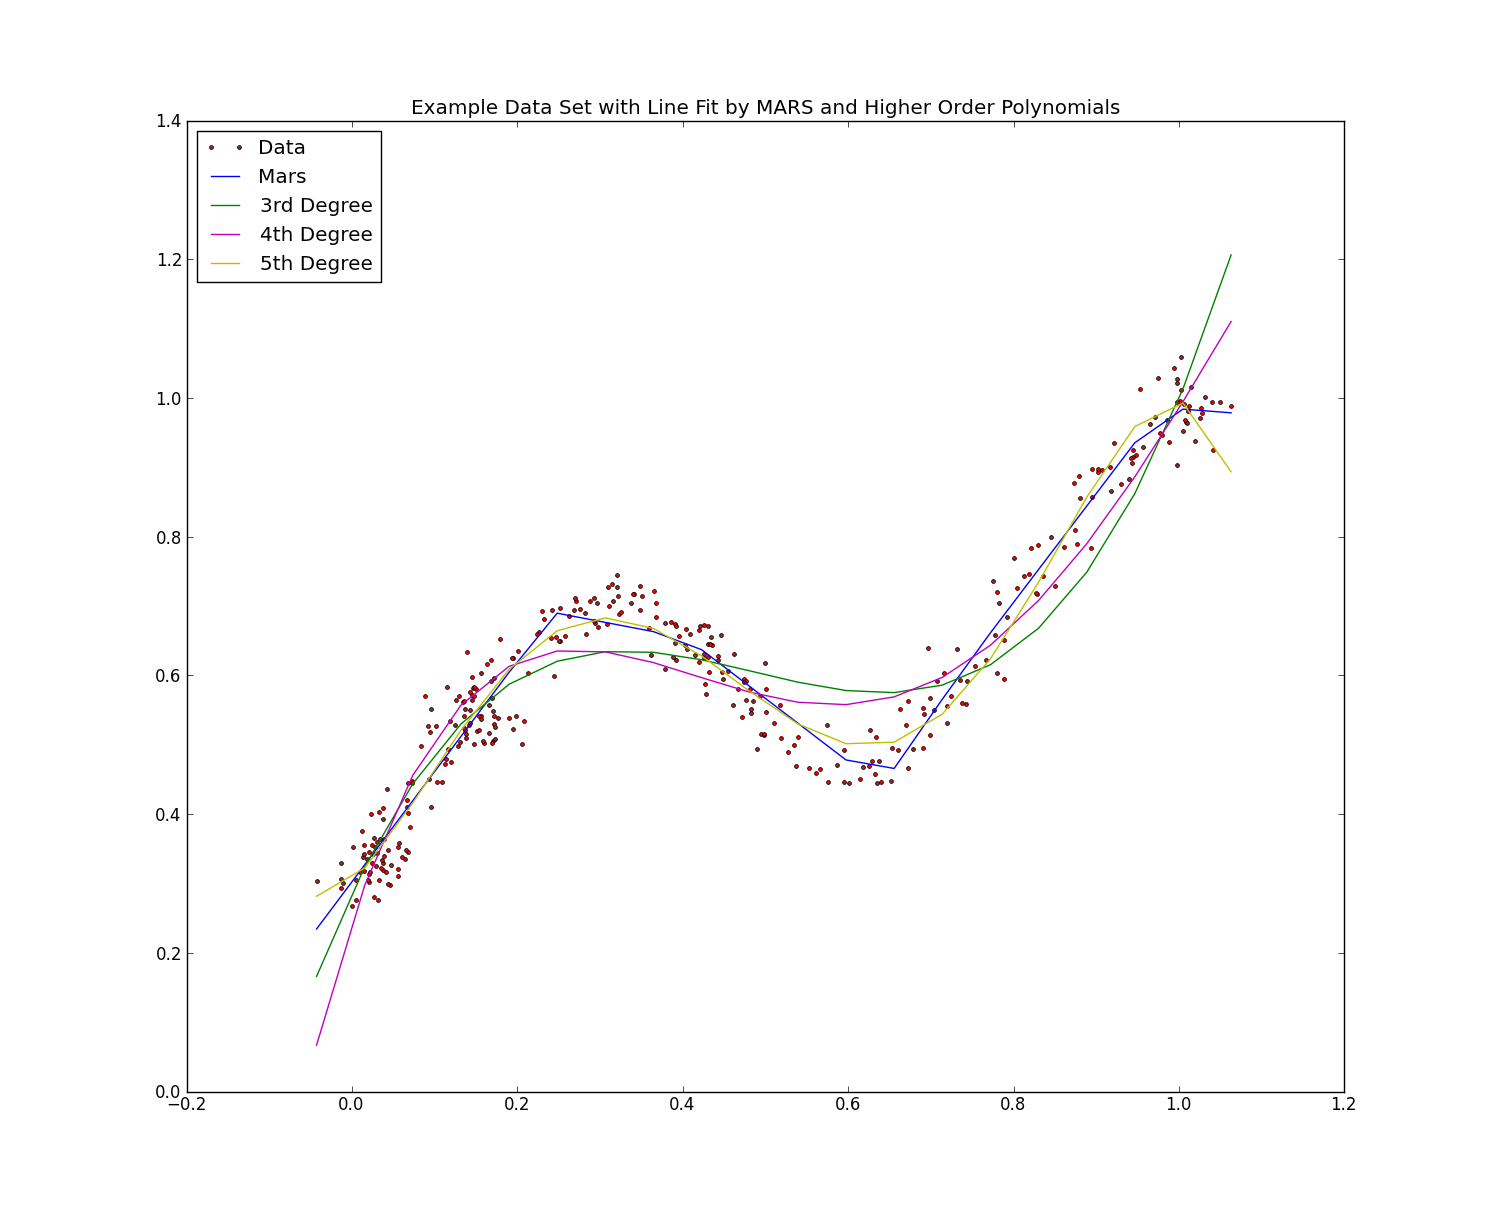
\includegraphics[width=6.5in]{example_data_poly_fit.png}
    \caption{Comparison of the Fit of Mars vs Polynomial Functions}
    \label{Example Data}
\end{figure}

As Figure 3 shows, visually it appears that the Mars model fitted via the Earth software has closer fit than the polynomial functions. Further, the reader should bear in mind that the fitting of the polynomial functions would not be automatic and requires manual input from the modeler, versus the Earth software which automatically selects the best model structure. To empirically test the fit of the 4 models, we define a function to compute the $RSS$. 

\begin{lstlisting}[caption={Calculate the $RSS$ for the Four Models  },label=lst:expected_times,firstnumber=63]
# Create function to calc RSS
def rss(y_obs, y_predicted):
    r=0
    for i in range(len(y_obs)):
        t=(y_obs[i]-y_predicted[i])**2.
        r=r+t
    return r

# Calc RSS for all models
y_predicted1=[earth_predictor([X[i], "?"]) for i in range(len(X))]
y_predicted3=pp3(X)
y_predicted4=pp4(X)
y_predicted5=pp5(X)

r1=rss(Y,y_predicted1)
r3=rss(Y,y_predicted3)
r4=rss(Y,y_predicted4)
r5=rss(Y,y_predicted5)
\end{lstlisting}

\begin{table}[H]
\caption{$RSS$ For the Four Models}
\centering
\begin{tabular}{c c}
\hline\hline
Method & $RSS$ \\
\hline
MARS & 0.59 \\
3rd Degree & 1.57 \\
4th Degree & 1.32 \\
5th Degree & 0.60 \\
\hline
\end{tabular}
\label{table:nonlin} 
\end{table}

As Table 1 shows, the MARS model has the lowest $RSS$, indicating superior fit as compared to the 3 other competing models.
